\documentclass[tikz,border=4pt]{standalone}
\usepackage{amsmath}
\usepackage{tikz}
\usetikzlibrary{arrows.meta,calc,decorations.markings}

\begin{document}
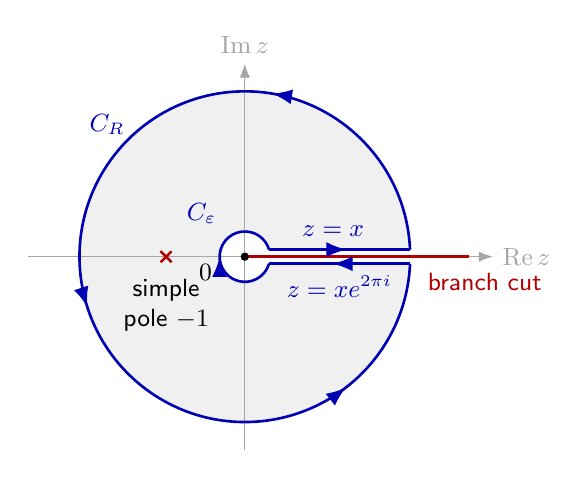
\begin{tikzpicture}[
  >=Latex,
  axis/.style={gray!70,->,line width=0.45pt},
  contour/.style={line width=0.95pt,blue!70!black},
  cut/.style={red!70!black,line width=1.2pt},
  note/.style={font=\small\sffamily}
]
  % Geometry: outer radius 2.1, inner radius 0.32, sides at y = +-0.09.
  % Intersections: outer (2.098, +-0.09) at angle 2.46 deg;
  %                inner (0.307, +-0.09) at angle 16.34 deg.

  % Enclosed region: outer disk minus the hole about the branch point.
  \fill[gray!12]
    (0.307,0.09) -- (2.098,0.09)
    arc[start angle=2.46,end angle=357.54,radius=2.1]
    -- (0.307,-0.09)
    arc[start angle=-16.34,end angle=-343.66,radius=0.32]
    -- cycle;

  \draw[axis] (-2.75,0) -- (3.15,0) node[right,note] {$\operatorname{Re}z$};
  \draw[axis] (0,-2.45) -- (0,2.45) node[above,note] {$\operatorname{Im}z$};

  % Branch cut along the positive real axis, straddled by the two sides.
  \draw[cut] (0.02,0) -- (2.85,0);
  \node[note,red!70!black,anchor=north west] at (2.2,-0.08) {branch cut};

  % Upper side: z = x, from epsilon out to R.
  \draw[contour,postaction={decorate},
    decoration={markings,mark=at position 0.55 with {\arrow{Latex}}}]
    (0.307,0.09) -- (2.098,0.09);
  % Outer circle C_R, counterclockwise.
  \draw[contour,postaction={decorate},
    decoration={markings,
      mark=at position 0.22 with {\arrow{Latex}},
      mark=at position 0.55 with {\arrow{Latex}},
      mark=at position 0.86 with {\arrow{Latex}}}]
    (2.098,0.09) arc[start angle=2.46,end angle=357.54,radius=2.1];
  % Lower side: z = x e^{2 pi i}, from R back to epsilon.
  \draw[contour,postaction={decorate},
    decoration={markings,mark=at position 0.55 with {\arrow{Latex}}}]
    (2.098,-0.09) -- (0.307,-0.09);
  % Inner circle C_epsilon, clockwise.
  \draw[contour,postaction={decorate},
    decoration={markings,mark=at position 0.5 with {\arrow{Latex}}}]
    (0.307,-0.09) arc[start angle=-16.34,end angle=-343.66,radius=0.32];

  \node[note,blue!70!black] at (1.12,0.33) {$z=x$};
  \node[note,blue!70!black] at (1.2,-0.38) {$z=xe^{2\pi i}$};
  \node[note,blue!70!black] at (-1.75,1.68) {$C_R$};
  \node[note,blue!70!black] at (-0.55,0.55) {$C_\varepsilon$};

  % Simple pole at z = -1, the only enclosed singularity.
  \draw[red!70!black,line width=0.9pt]
    (-1.07,-0.07)--(-0.93,0.07) (-1.07,0.07)--(-0.93,-0.07);
  \node[note,align=center] at (-1.0,-0.62) {simple\\pole $-1$};

  % Branch point kept outside by the hole.
  \fill (0,0) circle (1.5pt);
  \node[note] at (-0.5,-0.2) {$0$};
\end{tikzpicture}
\end{document}
